\documentclass[tikz,border=3mm]{standalone}
\usetikzlibrary{calc,arrows.meta}

\begin{document}
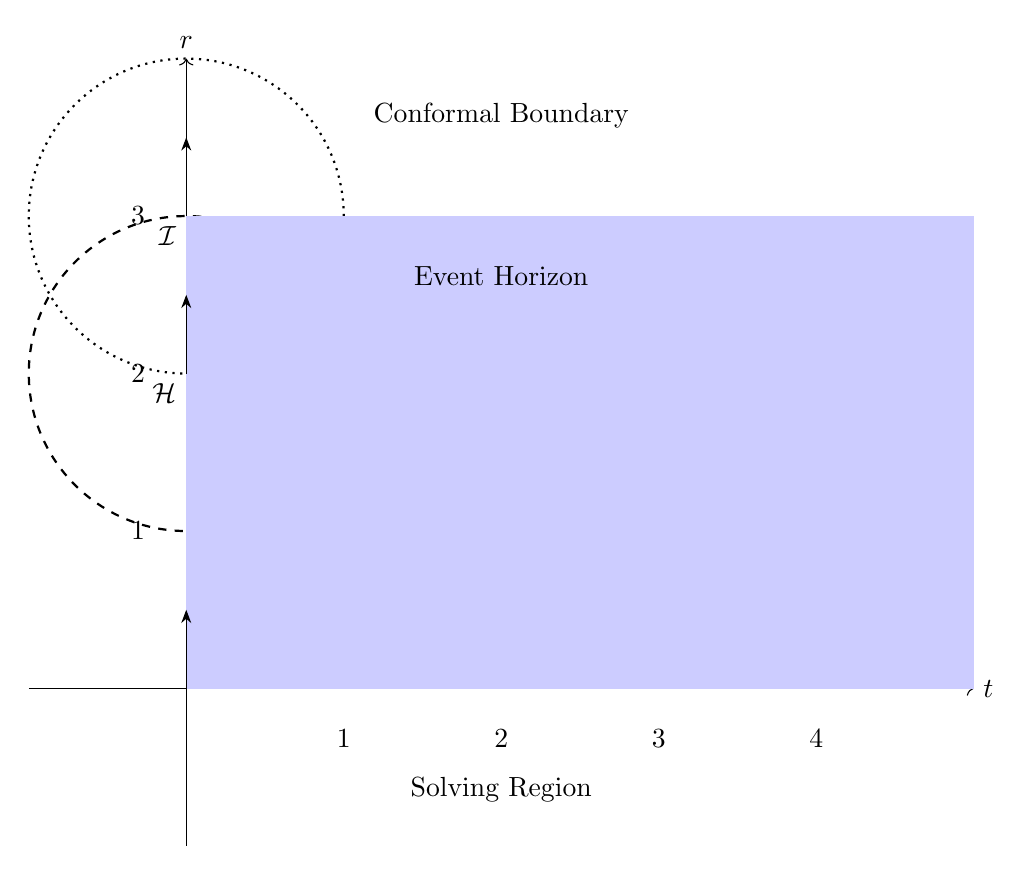
\begin{tikzpicture}[scale=2]
    % Draw the time axis
    \draw[->] (-1,0) -- (5,0) node[right] {$t$};
    
    % Draw the radial axis
    \draw[->] (0,-1) -- (0,4) node[above] {$r$};
    
    % Event Horizon
    \draw[dashed,thick] (0,2) circle[radius=1cm] node[below left] {$\mathcal{H}$};
    
    % Conformal Boundary
    \draw[dotted,thick] (0,3) circle[radius=1cm] node[below left] {$\mathcal{I}$};
    
    % Region where the wave equation is solved
    \fill[blue!20] (0,0) rectangle (5,3);
    
    % Labels for regions
    \node at (2,-0.5) [below] {Solving Region};
    \node at (2,3.5) [above] {Conformal Boundary};
    \node at (2,2.5) [above] {Event Horizon};
    
    % Arrows indicating the direction of time
    \draw[-Stealth] (0,0) -- (0,0.5);
    \draw[-Stealth] (0,3) -- (0,3.5);
    \draw[-Stealth] (0,2) -- (0,2.5);
    
    % Time labels
    \foreach \x in {1,2,3,4} {
        \node at (\x,-0.2) [below] {\x};
    }
    
    % Radial labels
    \foreach \y in {1,2,3} {
        \node at (-0.2,\y) [left] {\y};
    }
\end{tikzpicture}
\end{document}